\documentclass{assignment}
\usepackage{amsmath}
\usepackage{lipsum}
\usepackage{multicol}
\usepackage{fancyhdr}
\usepackage{graphicx}
\usepackage[dvipsnames]{xcolor}
\usepackage{enumitem}

\usepackage{color,soul}
\usepackage{amsfonts}
\def\code#1{\texttt{#1}}
\usepackage{graphicx} % Required for inserting images
\graphicspath{ {./images/} }
\usepackage{booktabs}
\usepackage{xcolor}
\usepackage{mdframed}
\usepackage{bbm}
\usepackage{hyperref}
\usepackage{bookmark} % Required for enhanced bookmarks
\usepackage{cleveref}

\begin{document}

\assignmentTitle{assets/kth-logo.png}
{Optimization}
{Homework 3}
{SF1811}
{Lucas Frykman, Jonathan Tadesse}
{Student personal numbers: 021012-7650, 970729-4311}
{Student Emails: lfrykman@kth.se, jtadesse@kth.se}
AI level 1: Used chatgpt to parse calculations in to latex, gave us easier to read documentation on
the \code{quadprog} function.
\\
In this assignment you are asked to formulate Markowitz model for portfolio optimization
as a quadratic optimization problem, and solve it using Matlab. 

The model can briefly be described as follows. A fraction $x_j$ of the total capital is invested
in asset $j$, $j=1,\dots,n$. The annual (or daily) return of each asset is modelled as a random
variable $\xi_j$. The random variables can be correlated and it is assumed that the expected
values $\mu_j := \mathbb{E}[\xi_j]$ and the covariance matrix $C_{ij} := \mathbb{E}[(\xi_i - \mu_i)(\xi_j - \mu_j)]$ are known,
$i,j=1,\dots,n$. The annual return of an asset is defined as the relative change of the asset
price in a year. For given expected returns $\mu = (\mu_1,\dots,\mu_n)^T$, given correlation matrix $C$
and a given expected return of the portfolio, $r$, Markowitz portfolio optimization problem
is then to determine $x = (x_1,\dots,x_n)^T$ that minimizes the variance of the portfolio subject
to the expected return $r$ being met. For a given $r$, we may formulate the problem as

\[
(P_r)\quad 
\begin{aligned}
&\underset{x\in\mathbb{R}^n}{\text{minimize}}   && \frac{1}{2} x^T C x \\
&\text{subject to} && \mu^T x = r, \\
&                  && e^T x = 1, \\
&                  && x \geq 0.
\end{aligned}
\]

where $e = (1,\dots,1)^T$. Please note that $(P_r)$ is a convex optimization problem, as the
covariance matrix $C$ is positive semidefinite and the constraints are linear. The reason for
considering $r$ as explicit parameter is that it is interesting to consider $(P_r)$ for a range of
$r$ values to see the tradeoff between the optimal value of $(P_r)$ and the return, as $r$ varies.

You are asked below to solve the problem $(P_r)$, and some variants of it, for $n=8$ and a
range of $r$ values, where $C$ and $\mu$ are generated by the Matlab file \texttt{hw3data.m}, which is
available in Canvas. The file uses the Matlab random number generator for generating the
data. You should initialize with a seed using the Matlab \texttt{rng} function, using one group
member's date of birth. State which seed you use in the report.
\\
Using Johnathan's personal number we obtained:
$$ C = 
\begin{bmatrix}
4.0000 & -2.3790 & 2.7513 & -2.5808 & 2.0819 & -2.0742 & 2.3145 & -2.4852 \\
-2.3790 & 5.6595 & -4.9089 & 4.0931 & -3.0954 & 2.9607 & -3.2119 & 3.3784 \\
2.7513 & -4.9089 & 17.0313 & -10.6508 & 7.1597 & -6.4200 & 6.6862 & -6.8374 \\
-2.5808 & 4.0931 & -10.6508 & 26.6426 & -13.4324 & 10.7063 & -10.4533 & 10.2621 \\
2.0819 & -3.0954 & 7.1597 & -13.4324 & 27.0889 & -16.1935 & 14.0540 & -12.9347 \\
-2.0742 & 2.9607 & -6.4200 & 10.7063 & -16.1935 & 38.7211 & -25.2040 & 20.6193 \\
2.3145 & -3.2119 & 6.6862 & -10.4533 & 14.0540 & -25.2040 & 65.6222 & -40.2639 \\
-2.4852 & 3.3784 & -6.8374 & 10.2621 & -12.9347 & 20.6193 & -40.2639 & 98.8191
\end{bmatrix} $$
$$ \mu = \left(\begin{array}{c} 3\\ 4\\ 5\\ 6\\ 7\\ 8\\ 9\\ 10 \end{array}\right)$$
\newpage
\section*{Exercise 3.1}
Consider problem $(P_r)$.

The optimality conditions for $(P_r)$ may be written as

\[
Cx - \mu u + ev - y = 0,
\]

\[
r - \mu^T x = 0,
\]

\[
e^T x - 1 = 0,
\]

\[
x \geq 0, \ y \geq 0, \ x_j y_j = 0, \ j=1,\ldots,n,
\]

where $x \in \mathbb{R}^n$, $u \in \mathbb{R}$, $v \in \mathbb{R}$, and $y \in \mathbb{R}^n$.

Using the \code{quadprog} function we obtained the following plot \Cref{fig1}.

\begin{figure}[htbp]
    \centering
        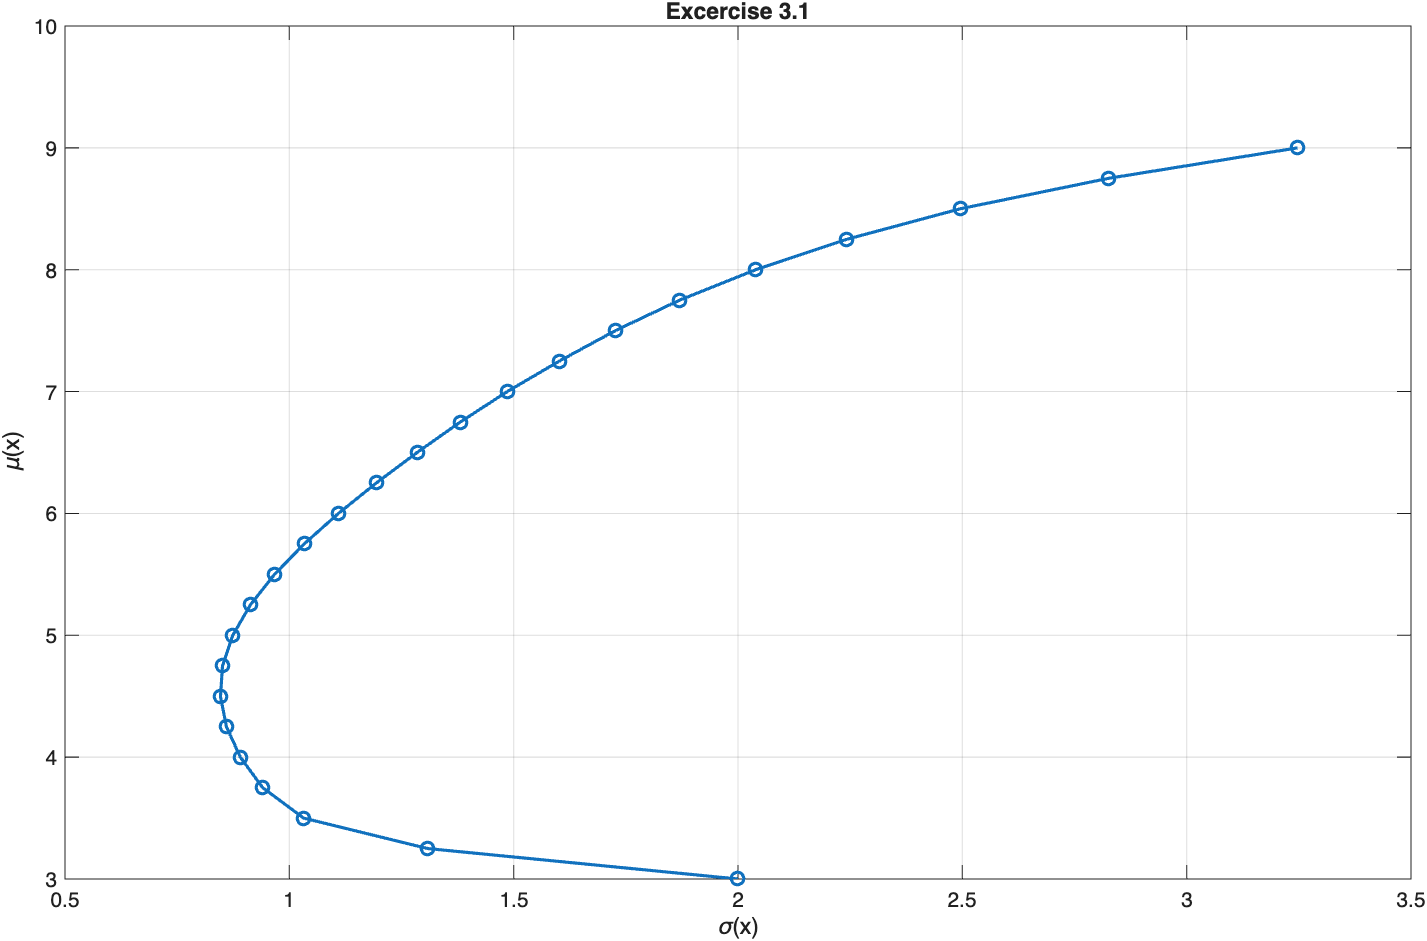
\includegraphics[width=0.8\textwidth]{assets/excercise1}
        \caption{Markowitz Efficient Frontier}
        \label{fig1}
\end{figure}
\newpage
\section*{Exercise 3.2}
\subsection*{(a)}
When in the original problem $e^T x = 1$, we invest all capital among the $n$ assets.
If we switch to $e^T x \leq 1$, we allow less than 100\% of the capital to be invested.
Any uninvested portion $1 - \sum_{j} x_j$ remains risk-free at zero return and zero variance (bank account). Thus,

\[
e^T x = 1 \;\longrightarrow\; e^T x \leq 1
\]

models the scenario when we don't invest the entire budget.
If $\sum_{j} x_j = 1$, we invested fully; if $\sum_{j} x_j < 1$, the remainder is uninvested.
\subsection*{(b)}
Let $(x^*,u^*,v^*,y^*)$ be an optimal solution to the original problem

\[
\begin{array}{ll}
\min & \dfrac{1}{2}x^T Cx \\[6pt]
\text{subject to} & \mu^T x = r, \quad e^T x =1, \quad x\geq 0
\end{array}
\]

with Lagrange multipliers $u^* \in \mathbb{R}$ and $y^* \in \mathbb{R}_{\geq 0}^n$. We consider now the
modified problem:

\[
\begin{array}{ll}
\min & \dfrac{1}{2}x^T Cx \\[6pt]
\text{subject to} & \mu^T x = r, \quad e^T x \leq 1, \quad x\geq 0
\end{array}
\]

We need to show that the modified problem satisfies the following:

\begin{enumerate}
\item Primal feasibility
\item Dual feasibility
\item Stationarity
\item Complementary slackness
\end{enumerate}

\begin{enumerate}
\item Primal Feasibility: Since $e^Tx^*=1$ in the original solution, we immediately have $e^Tx^* \leq 1$ for the modified problem. Hence $x^*$ is feasible.
\item Dual Feasibility: In this problem we have a dual inequality constraint $v\geq 0$ this is satisfied if we set $v=0$.
\item Complementary Slackness: In the modified problem, $(e^Tx^*-1)v^*=0$. But $e^Tx^*-1$ implies $(1-1)v^*=0$ is automatically satisfied. Likewise, $x_j^*y_j^*=0$ still holds from the original solution.
\item Stationarity:
\[
Cx^* - \mu u^* + ev^* - y^* = 0.
\]
\end{enumerate}

So all the KKT conditions for the modified problem are satisfied by $(x^*,u^*,v^*,y^*)$ if $v^*\geq0$. This means $x^*$ is also optimal in the modified problem.

\subsection*{(c)}
\begin{figure}[htbp]
    \centering
        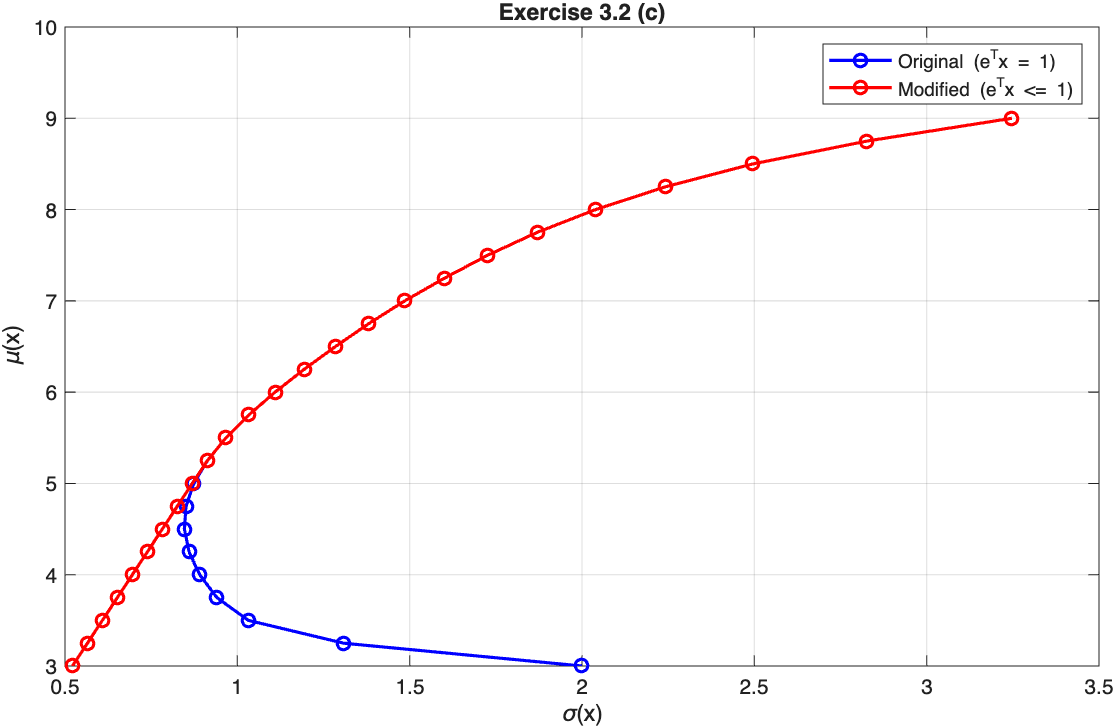
\includegraphics[width=0.8\textwidth]{assets/exercise2}
        \caption{Markowitz Efficient Frontier Original vs modified}
        \label{fig2}
\end{figure}

We modify the original Markowitz model by replacing the constraint

$$e^T x = 1$$

with 

$$e^T x \leq 1$$

Wherever (see \Cref{fig2}) the red points lie to the left (lower $\sigma(x) = \sqrt{x^TCx}$) for the same $\mu (x) = \mu^T x$, we see reduced risk
by not investing the full budget. However for many target returns the curves coincide, which means that fully investing 
remains optimal there. Therefore if we have $e^T x\leq 1$ we can only improve or match the original risk-return tradeoff but never
worsen it.

\section*{Exercise 3.3}

\subsection*{(a)}
If we change $\mu^T x = r$ to $\mu^T x \geq r$, we now require the portfolio's expected return to be at least $r$ instead of exactly $r$. This represents imposing a minimum acceptable return rather than a fixed target.
\subsection*{(b)}
Now assume that $(x^*,u^*,v^*,y^*)$ already solves the original problem $P_r$, so $\mu^T x^* = r$. We want to check if it also solves the modified problem.

1. Primal feasibility:

We need $\mu^T x^* \geq r$. Since $\mu^T x^* = r$, we have $\mu^T x^* - r = 0 \geq 0$. So that holds. We also have $e^T x^* = 1$ (same as before) and $x^* \geq 0$. So the primal feasibility is satisfied.

2. Complementary slackness $(r - \mu^T x^*) u^* = 0$:

From the original solution, $\mu^T x^* = r$. Hence $r - \mu^T x^* = 0$. Multiplying by any $u^*$ (with $u^* \geq 0$) gives $0 \cdot u^* = 0$. So complementary slackness is satisfied.

3. Dual feasibility:

In this problem, the constraint $\mu^T x \geq r$ requires $u^* \geq 0$. If $u^* = 0$, this satisfies the condition. If $u^* > 0$, it also satisfies $u^* \geq 0$. Therefore, dual feasibility is satisfied.

4. Stationarity: The stationarity condition for the modified problem is:
\[
Cx^* - \mu u^* + ev^* - y^* = 0
\]
In the original problem, stationarity required: $Cx^* - \mu u^* + ev^* - y^* = 0$

These are identical.
\subsection*{(c)}
\begin{figure}[htbp]
    \centering
        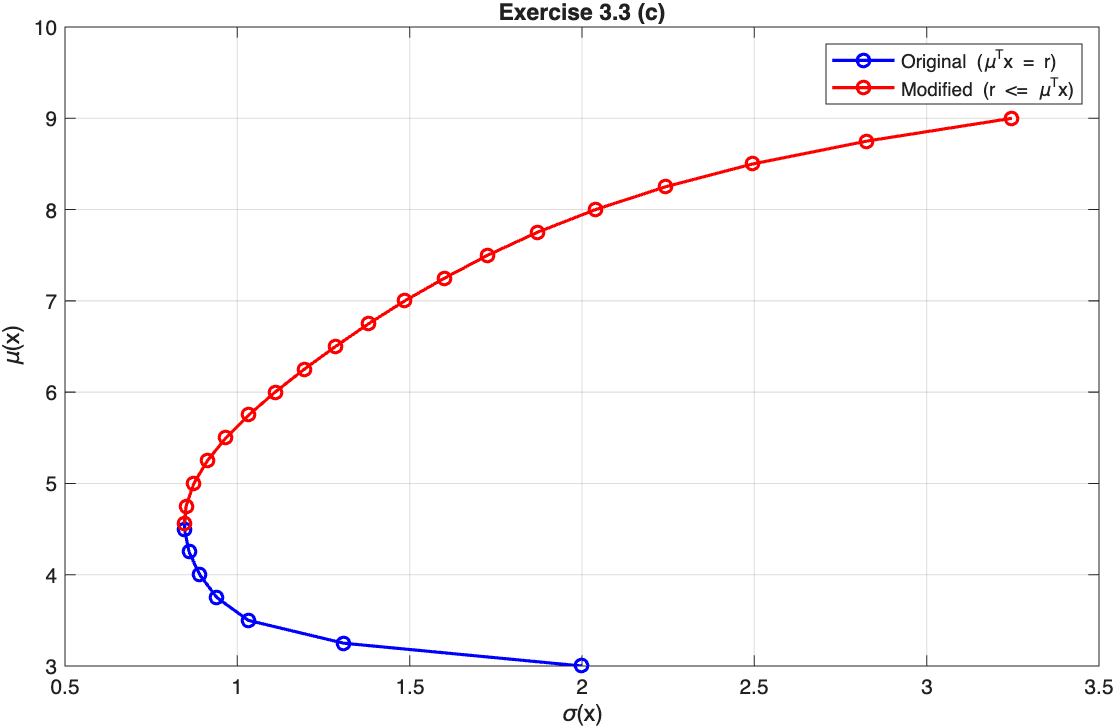
\includegraphics[width=0.8\textwidth]{assets/exercise3c}
        \caption{Markowitz Efficient Frontier Original vs modified 3.3(c)}
        \label{3.3c}
\end{figure}


Since we now allow our portfolio to exceed the target return r, we initially expected a different efficient frontier.
However we seet that both frontiers largely coincide. Meaning the optimal solution for the modified problem gains 
little by exceeding r. Even though the modified problem is more flexible (since we have $\mu^Tx >r$), this
flexibility does not help if pushing return above r substantially increases risk. Thus the solution often stays at
$\mu^T x= r$, and both frontiers eventually coincide. 


\section*{Exercise 3.4}

\subsection*{(a)}
In the original markowitz portfolio problem, the rule $x_j \geq 0$ means that the fraction of money allocated to each asset
j must be non-negative. Which basically means we can only "buy" or "invest in" an asset but we can't "borrow and sell" (i.e no short selling).

Short selling asset $j$ basically means borrowing shares of that asset, selling them at the current market price, and then 
repurchasing them later to return to the lender. A negative value $x_j \le 0$ represents this operation of borrowing and
selling. \\
If we remove the constraint $x_j \geq 0$, it is now mathematically possible to have $x_j \le 0$. \\
Which we interpret financially as: \\
$x_j \ge 0$: a long position in asset $j$. \\
$x_j \le$: a short position in asset $j$.
\subsection*{(b)}

Let $(x^*, u^*, v^*, y^*)$ be an optimal solution for the original problem

$$\min_{x \geq 0} \frac{1}{2} x^T C x \text{ subject to } \mu^Tx = r, e^Tx = 1$$

with corresponding KKT conditions:
\begin{enumerate}
    \item Stationarity  
        $$Cx^* - \mu u^* - ev^* - y^* = 0$$
    \item Primal feasibility: 
        $$\mu^T x^* = r, e^Tx^* = 1, x^*\geq 0$$
    \item Dual Feasibility
        $$y^* \geq 0$$
    \item Complementary slackness
        $$x^*_jy^*_j = 0, \text{ for all } j$$
\end{enumerate}
Now we remove $x \geq 0$ to allow short selling. The new problem has no nnonegativity constraints, its KKT conditions are simply:

\begin{enumerate}
    \item Stationary 
        $$Cx^* - \mu^* -ev^* = 0$$
    \item Primal feasibility 
        $$\mu^T x^* = r, e^Tx^* = 1$$
\end{enumerate}

If $y^*=0$ in the original solution, then: From original stationarity, $Cx^* - \mu u^* - ev^* - y^* = 0$
becomes $Cx^* - \mu^* -ev^* = 0$ once $y^* = 0$. THe same $(x^*, u^*, v^*)$  satisfies the new stationary condition. 
$\mu^T x^* = r, e^Tx^* = 1$ are still valid, so primal feasibility holds.

Hence $(x^*, u^*, v^*)$  is also optimal for the short-sale-allowed problem.


\subsection*{(c)}
\begin{figure}[htbp]
    \centering
        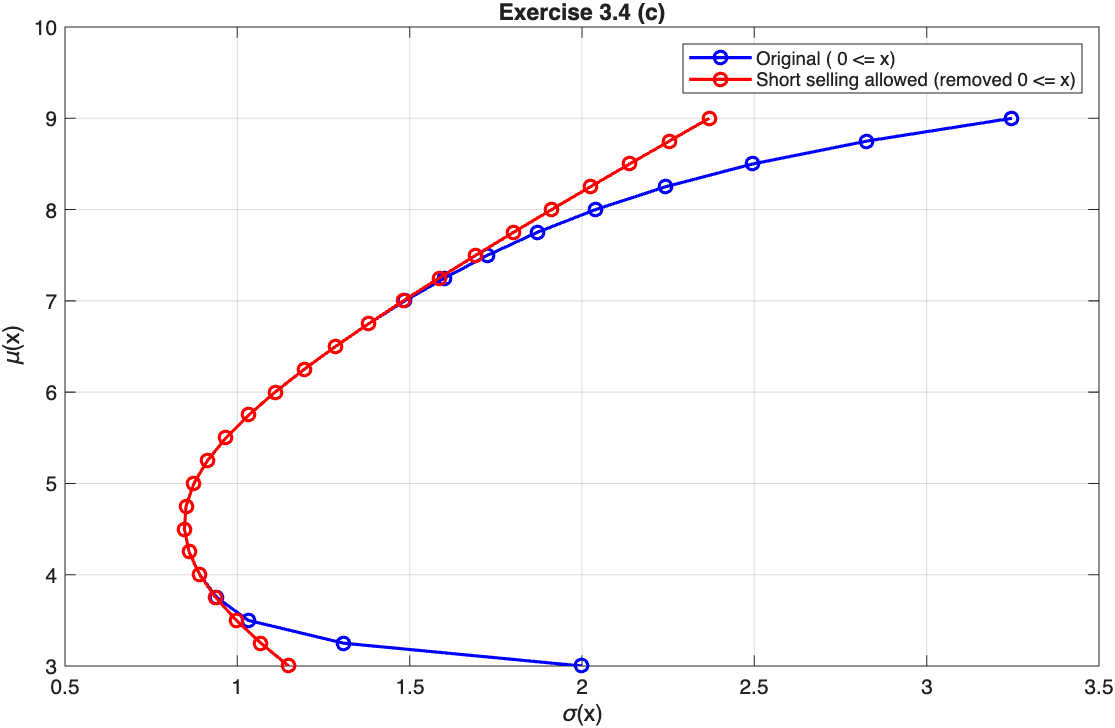
\includegraphics[width=0.8\textwidth]{assets/exercise4c}
        \caption{Markowitz Efficient Frontier Original vs short selling allowed 3.4(c)}
        \label{3.4c}
\end{figure}
At small enough risk (i.e small $\sigma<1$ ), the red and blue curves coincide, meaning short selling doesn't help for those returns.
However at higher returns the red curve shifts up or left which means it acheives higher return for the same risk or lower
risk for the same return. Because short selling expands the set of portfolios, its frontier
can only match or outperform the long-only frontier.

\end{document}
